\documentclass[]{report}


% Title Page
\title{Homework II Solutions \\ of \\ \emph{Advanced Mechanical Vibrations} class.}
\author{Burak ER}

\usepackage{psfrag}

\usepackage{amsmath}

\usepackage{amssymb}

\usepackage{pstricks, pst-node, pst-plot, pst-circ}

\usepackage{moredefs}

\usepackage{hyperref}

\usepackage{cleveref}

\usepackage{graphicx}

\usepackage{epstopdf}

\usepackage{epsfig}

\usepackage{algorithm}

\usepackage{program}

\usepackage{graphicx}

\usepackage{caption}

\usepackage{subcaption}

\usepackage[autolinebreaks,useliterate]{mcode}

\crefname{lstlisting}{listing}{listings}

\Crefname{lstlisting}{Listing}{Listings}

\begin{document}


\maketitle
\begin{abstract}
Includes the solutions for the first homework problems of \emph{Advanced Mechanical Engineering} class given at Bursa Technical University, in fall semester 2013.
\\
\\
Written by \LaTeX ~using TeXstudio...
\end{abstract}
\section*{Problem 1}
Half-car model of a vehicle is given in the \cref{fig:2st_Assignment}. The physical properties are as follows: $m=420kg$, $m1=m2=53kg$, $I_x=820 kgm^2$, $b_1=0.7m$, $b_2=0.75m$, $k =10000Nm^{-1}$, $k_t=200000 Nm^{-1}$, $kR=25000 Nm^{-1}$, $k_4= 1972900 Nm^{-1}$, $c=200 Nsm^{-1}$. The vehicle is subject to base motions $y_1$ and $y_2$.

\begin{figure}[ht!]
\begin{subfigure}[b]{0.5\textwidth}
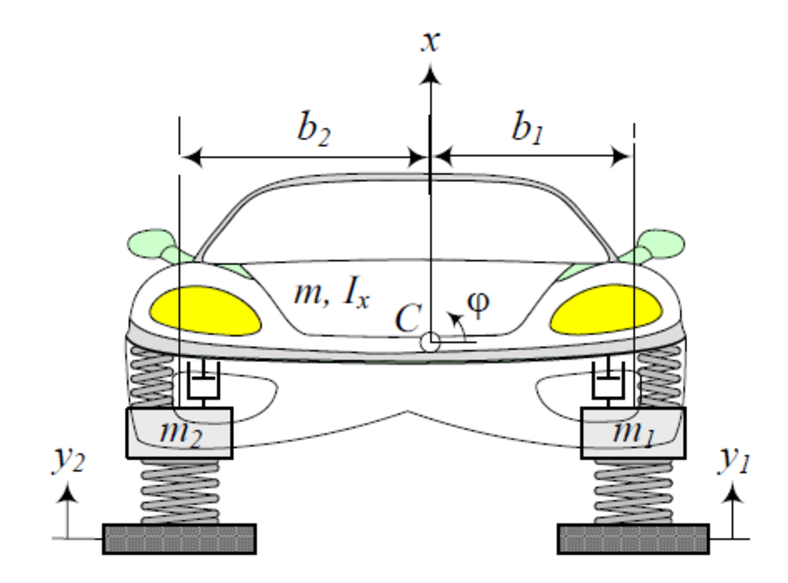
\includegraphics[width=\textwidth]{./Figures/2st_Assignment} \caption{whole car body}
\end{subfigure}~
\begin{subfigure}[b]{0.5\textwidth}
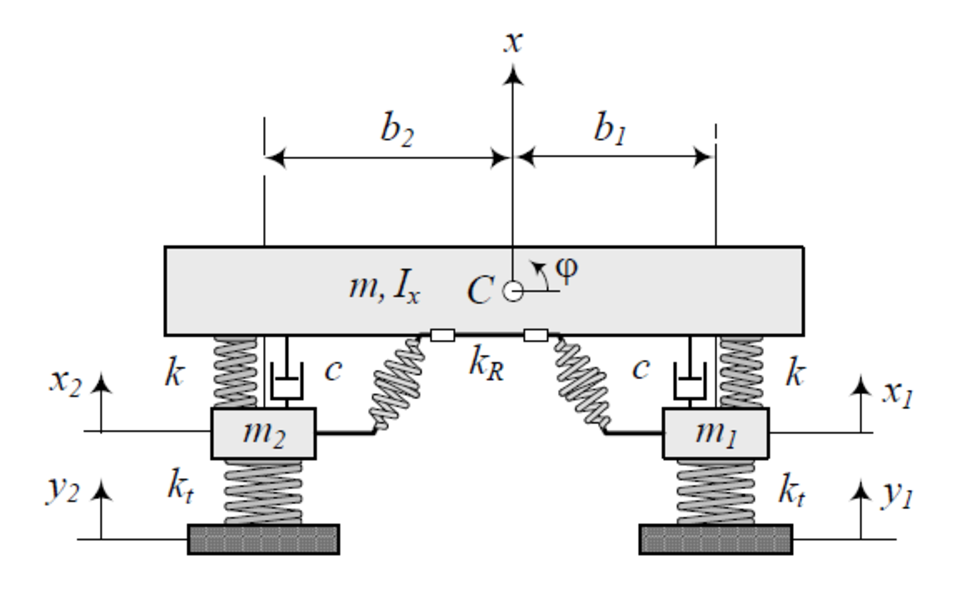
\includegraphics[width=\textwidth]{./Figures/2st_Assignment_1}
\caption{equivalent model}
\end{subfigure}
\caption{problem 1}
\label{fig:2st_Assignment}
\end{figure}
Mass, damping and stiffness matrices of the car model are
\begin{eqnarray*}
\mathbf{M}=\left[\begin{array}{cccc}
m&0&0&0\\
0&I_x&0&0 \\
0&0&m_1&0 \\
0&0&0&m_2
\end{array}\right]
\end{eqnarray*}

\begin{eqnarray*}
\mathbf{C}=\left[\begin{array}{cccc}
2c&cb_1-cb_2&-c&-c\\
cb_1-cb_2&cb_1^2+cb_2^2&-cb_1&cb_2 \\
-c&-cb_1&c&0 \\
-c&cb_2&0&c
\end{array}\right]
\end{eqnarray*}

\begin{eqnarray*}
\mathbf{K}=\left[\begin{array}{cccc}
2k&kb_1-kb_2&-k&-k\\
kb_1-kb_2&kb_1^2+kb_2^2&-kb_1&kb_2 \\
-k&-kb_1&k+k_t&0 \\
-k&kb_2&0&k+k_t
\end{array}\right]
\end{eqnarray*}

\subsection*{Question 1}

\begin{enumerate}
\item Find the undamped natural frequencies and vibration modes by
\begin{enumerate}
\item Solving characteristic polynomial.
\item Matrix iteration method.
\end{enumerate}
\item Plot the vibration modes, comment them and make conclusions.
\item Compute modal mass and stiffness values.
\item Show that vibration modes are orthogonal to each other with respect to mass and stiffness matrices.
\end{enumerate}

\begin{center}
\subsection*{Solution 1}
\end{center}
\textbf{Solving characteristic polynomial.}\\~\\
Undamped system characteristic polynominal is found from the equation
\begin{eqnarray*}
\mathrm{det}\left(-\lambda^2\mathbf{M}+ \mathbf{K}\right)=0
\end{eqnarray*}
which is found 
\begin{eqnarray*}
9.67\cdot 10^8\, {\mathrm{\lambda}}^8 - 7.75\cdot 10^{12}\, {\mathrm{\lambda}}^6 + 1.59\cdot 10^{16}\, {\mathrm{\lambda}}^4 - 1.35\cdot 10^{18}\, {\mathrm{\lambda}}^2 + 2.94\cdot 10^{19}=0
\end{eqnarray*}
where the solution of natural frequencies are found as
\begin{eqnarray*}
{\mathbf{\Lambda}}=\left[\begin{array}{c} 62.964\\ 62.951\\ 6.749\\6.517 \end{array}\right]\mathrm{radian/s}
\end{eqnarray*}
\emph{I}th mode shape of the system can be found by substituting $\lambda_i$ on the equation 
\begin{eqnarray*}
\left(-\lambda^2\mathbf{M}+ \mathbf{K}\right)\mathbf{u}=\mathbf{0}
\end{eqnarray*}
that is found 
\begin{eqnarray*}
\begin{array}{ccc} 500.0\, u_{2} + 10000.0\, u_{3} + 10000.0\, u_{4} + u_{1}\, \left(420.0\, {\mathrm{\lambda}_i}^2 - 20000.0\right)&=& 0\\ 500.0\, u_{1} + 7000.0\, u_{3} - 7500.0\, u_{4} + u_{2}\, \left(820.0\, {\mathrm{\lambda}_i}^2 - 35525.0\right)&=& 0\\ 10000.0\, u_{1} + 7000.0\, u_{2} + u_{3}\, \left(53.0\, {\mathrm{\lambda}_i}^2 - 210000.0\right)&=& 0\\ 10000.0\, u_{1} - 7500.0\, u_{2} + u_{4}\, \left(53.0\, {\mathrm{\lambda}_i}^2 - 210000.0\right)&=& 0 \end{array}
\end{eqnarray*}
with assuming $u_1=1$ and then normalizing the mode shapes, mode shapes are are found as\\~\\
for $\lambda_1$
\begin{eqnarray*}
\mathbf{u}_1=\left[\begin{array}{cccc} 0.00859  \\ 0.00011  \\ 0.97766  \\ 0.36874 \end{array}\right]
\end{eqnarray*}
for $\lambda_2$
\begin{eqnarray*}
\mathbf{u}_2=\left[\begin{array}{cccc} -0.00015  \\ 0.0031884  \\ -0.19903  \\ 0.92811 \end{array}\right]
\end{eqnarray*}
for $\lambda_3$
\begin{eqnarray*}
\mathbf{u}_3=\left[\begin{array}{cccc} -0.69795  \\ -0.71612 \\ 0.04038  \\ 0.04902\end{array}\right]
\end{eqnarray*}
for $\lambda_4$
\begin{eqnarray*}
\mathbf{u}_4=\left[\begin{array}{cccc} -0.71609 \\ 0.6979  \\ 0.05428  \\ -0.01575 \end{array}\right]
\end{eqnarray*}
\\~\\
\textbf{Plot the vibration modes, comment them and make conclusions.}
\\~\\
Plot of vibration modes is given in \cref{fig:allmodes}. What can be seen from the figure is; the dominant term in the first and second mode are displacements of the tires. These modes have two highest natural frequencies. In the third and fourth mode the dominant variables are displacement and the rotation of the car body. These modes have the lowest two natural frequencies.
\\~\\
It is concluded that, as expected, low frequency modes exist just because of the contribution of the body of the car and high frequency modes exist because of the contribution of the tires.
\begin{figure}[h!]
\centering
% This file is generated by the MATLAB m-file laprint.m. It can be included
% into LaTeX documents using the packages graphicx, color and psfrag.
% It is accompanied by a postscript file. A sample LaTeX file is:
%    \documentclass{article}\usepackage{graphicx,color,psfrag}
%    \begin{document}% This file is generated by the MATLAB m-file laprint.m. It can be included
% into LaTeX documents using the packages graphicx, color and psfrag.
% It is accompanied by a postscript file. A sample LaTeX file is:
%    \documentclass{article}\usepackage{graphicx,color,psfrag}
%    \begin{document}% This file is generated by the MATLAB m-file laprint.m. It can be included
% into LaTeX documents using the packages graphicx, color and psfrag.
% It is accompanied by a postscript file. A sample LaTeX file is:
%    \documentclass{article}\usepackage{graphicx,color,psfrag}
%    \begin{document}\input{allmode}\end{document}
% See http://www.mathworks.de/matlabcentral/fileexchange/loadFile.do?objectId=4638
% for recent versions of laprint.m.
%
% created by:           LaPrint version 3.16 (13.9.2004)
% created on:           05-Jan-2014 21:04:15
% eps bounding box:     15 cm x 8.8506 cm
% comment:              
%
\begin{psfrags}%
\psfragscanon%
%
% text strings:
\psfrag{s01}[b][b]{\color[rgb]{0,0,0}\setlength{\tabcolsep}{0pt}\begin{tabular}{c}mode 1\end{tabular}}%
\psfrag{s02}[b][b]{\color[rgb]{0,0,0}\setlength{\tabcolsep}{0pt}\begin{tabular}{c}relative displacement\end{tabular}}%
\psfrag{s05}[b][b]{\color[rgb]{0,0,0}\setlength{\tabcolsep}{0pt}\begin{tabular}{c}mode 3\end{tabular}}%
\psfrag{s07}[b][b]{\color[rgb]{0,0,0}\setlength{\tabcolsep}{0pt}\begin{tabular}{c}relative displacement\end{tabular}}%
\psfrag{s09}[b][b]{\color[rgb]{0,0,0}\setlength{\tabcolsep}{0pt}\begin{tabular}{c}mode 4\end{tabular}}%
\psfrag{s11}[b][b]{\color[rgb]{0,0,0}\setlength{\tabcolsep}{0pt}\begin{tabular}{c}relative displacement\end{tabular}}%
\psfrag{s13}[b][b]{\color[rgb]{0,0,0}\setlength{\tabcolsep}{0pt}\begin{tabular}{c}mode 2\end{tabular}}%
\psfrag{s15}[b][b]{\color[rgb]{0,0,0}\setlength{\tabcolsep}{0pt}\begin{tabular}{c}relative displacement\end{tabular}}%
%
% xticklabels:
\psfrag{x01}[t][t]{0}%
\psfrag{x02}[t][t]{0.1}%
\psfrag{x03}[t][t]{0.2}%
\psfrag{x04}[t][t]{0.3}%
\psfrag{x05}[t][t]{0.4}%
\psfrag{x06}[t][t]{0.5}%
\psfrag{x07}[t][t]{0.6}%
\psfrag{x08}[t][t]{0.7}%
\psfrag{x09}[t][t]{0.8}%
\psfrag{x10}[t][t]{0.9}%
\psfrag{x11}[t][t]{1}%
\psfrag{x12}[t][t]{1}%
\psfrag{x13}[t][t]{1.5}%
\psfrag{x14}[t][t]{2}%
\psfrag{x15}[t][t]{2.5}%
\psfrag{x16}[t][t]{3}%
\psfrag{x17}[t][t]{3.5}%
\psfrag{x18}[t][t]{4}%
\psfrag{x19}[t][t]{1}%
\psfrag{x20}[t][t]{2}%
\psfrag{x21}[t][t]{3}%
\psfrag{x22}[t][t]{4}%
\psfrag{x23}[t][t]{1}%
\psfrag{x24}[t][t]{2}%
\psfrag{x25}[t][t]{3}%
\psfrag{x26}[t][t]{4}%
\psfrag{x27}[t][t]{1}%
\psfrag{x28}[t][t]{2}%
\psfrag{x29}[t][t]{3}%
\psfrag{x30}[t][t]{4}%
%
% yticklabels:
\psfrag{v01}[r][r]{0}%
\psfrag{v02}[r][r]{0.1}%
\psfrag{v03}[r][r]{0.2}%
\psfrag{v04}[r][r]{0.3}%
\psfrag{v05}[r][r]{0.4}%
\psfrag{v06}[r][r]{0.5}%
\psfrag{v07}[r][r]{0.6}%
\psfrag{v08}[r][r]{0.7}%
\psfrag{v09}[r][r]{0.8}%
\psfrag{v10}[r][r]{0.9}%
\psfrag{v11}[r][r]{1}%
\psfrag{v12}[r][r]{-1}%
\psfrag{v13}[r][r]{-0.5}%
\psfrag{v14}[r][r]{0}%
\psfrag{v15}[r][r]{0.5}%
\psfrag{v16}[r][r]{1}%
\psfrag{v17}[r][r]{-1}%
\psfrag{v18}[r][r]{-0.5}%
\psfrag{v19}[r][r]{0}%
\psfrag{v20}[r][r]{0.5}%
\psfrag{v21}[r][r]{1}%
\psfrag{v22}[r][r]{-1}%
\psfrag{v23}[r][r]{-0.5}%
\psfrag{v24}[r][r]{0}%
\psfrag{v25}[r][r]{0.5}%
\psfrag{v26}[r][r]{1}%
\psfrag{v27}[r][r]{-1}%
\psfrag{v28}[r][r]{-0.5}%
\psfrag{v29}[r][r]{0}%
\psfrag{v30}[r][r]{0.5}%
\psfrag{v31}[r][r]{1}%
%
% Figure:
\resizebox{12cm}{!}{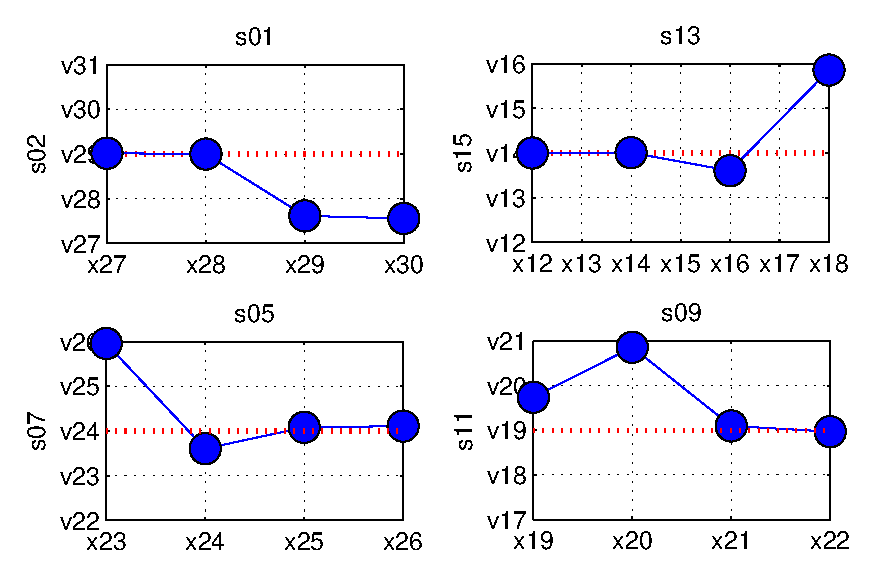
\includegraphics{./Figures/allmode.eps}}%
\end{psfrags}%
%
% End allmode.tex
\end{document}
% See http://www.mathworks.de/matlabcentral/fileexchange/loadFile.do?objectId=4638
% for recent versions of laprint.m.
%
% created by:           LaPrint version 3.16 (13.9.2004)
% created on:           05-Jan-2014 21:04:15
% eps bounding box:     15 cm x 8.8506 cm
% comment:              
%
\begin{psfrags}%
\psfragscanon%
%
% text strings:
\psfrag{s01}[b][b]{\color[rgb]{0,0,0}\setlength{\tabcolsep}{0pt}\begin{tabular}{c}mode 1\end{tabular}}%
\psfrag{s02}[b][b]{\color[rgb]{0,0,0}\setlength{\tabcolsep}{0pt}\begin{tabular}{c}relative displacement\end{tabular}}%
\psfrag{s05}[b][b]{\color[rgb]{0,0,0}\setlength{\tabcolsep}{0pt}\begin{tabular}{c}mode 3\end{tabular}}%
\psfrag{s07}[b][b]{\color[rgb]{0,0,0}\setlength{\tabcolsep}{0pt}\begin{tabular}{c}relative displacement\end{tabular}}%
\psfrag{s09}[b][b]{\color[rgb]{0,0,0}\setlength{\tabcolsep}{0pt}\begin{tabular}{c}mode 4\end{tabular}}%
\psfrag{s11}[b][b]{\color[rgb]{0,0,0}\setlength{\tabcolsep}{0pt}\begin{tabular}{c}relative displacement\end{tabular}}%
\psfrag{s13}[b][b]{\color[rgb]{0,0,0}\setlength{\tabcolsep}{0pt}\begin{tabular}{c}mode 2\end{tabular}}%
\psfrag{s15}[b][b]{\color[rgb]{0,0,0}\setlength{\tabcolsep}{0pt}\begin{tabular}{c}relative displacement\end{tabular}}%
%
% xticklabels:
\psfrag{x01}[t][t]{0}%
\psfrag{x02}[t][t]{0.1}%
\psfrag{x03}[t][t]{0.2}%
\psfrag{x04}[t][t]{0.3}%
\psfrag{x05}[t][t]{0.4}%
\psfrag{x06}[t][t]{0.5}%
\psfrag{x07}[t][t]{0.6}%
\psfrag{x08}[t][t]{0.7}%
\psfrag{x09}[t][t]{0.8}%
\psfrag{x10}[t][t]{0.9}%
\psfrag{x11}[t][t]{1}%
\psfrag{x12}[t][t]{1}%
\psfrag{x13}[t][t]{1.5}%
\psfrag{x14}[t][t]{2}%
\psfrag{x15}[t][t]{2.5}%
\psfrag{x16}[t][t]{3}%
\psfrag{x17}[t][t]{3.5}%
\psfrag{x18}[t][t]{4}%
\psfrag{x19}[t][t]{1}%
\psfrag{x20}[t][t]{2}%
\psfrag{x21}[t][t]{3}%
\psfrag{x22}[t][t]{4}%
\psfrag{x23}[t][t]{1}%
\psfrag{x24}[t][t]{2}%
\psfrag{x25}[t][t]{3}%
\psfrag{x26}[t][t]{4}%
\psfrag{x27}[t][t]{1}%
\psfrag{x28}[t][t]{2}%
\psfrag{x29}[t][t]{3}%
\psfrag{x30}[t][t]{4}%
%
% yticklabels:
\psfrag{v01}[r][r]{0}%
\psfrag{v02}[r][r]{0.1}%
\psfrag{v03}[r][r]{0.2}%
\psfrag{v04}[r][r]{0.3}%
\psfrag{v05}[r][r]{0.4}%
\psfrag{v06}[r][r]{0.5}%
\psfrag{v07}[r][r]{0.6}%
\psfrag{v08}[r][r]{0.7}%
\psfrag{v09}[r][r]{0.8}%
\psfrag{v10}[r][r]{0.9}%
\psfrag{v11}[r][r]{1}%
\psfrag{v12}[r][r]{-1}%
\psfrag{v13}[r][r]{-0.5}%
\psfrag{v14}[r][r]{0}%
\psfrag{v15}[r][r]{0.5}%
\psfrag{v16}[r][r]{1}%
\psfrag{v17}[r][r]{-1}%
\psfrag{v18}[r][r]{-0.5}%
\psfrag{v19}[r][r]{0}%
\psfrag{v20}[r][r]{0.5}%
\psfrag{v21}[r][r]{1}%
\psfrag{v22}[r][r]{-1}%
\psfrag{v23}[r][r]{-0.5}%
\psfrag{v24}[r][r]{0}%
\psfrag{v25}[r][r]{0.5}%
\psfrag{v26}[r][r]{1}%
\psfrag{v27}[r][r]{-1}%
\psfrag{v28}[r][r]{-0.5}%
\psfrag{v29}[r][r]{0}%
\psfrag{v30}[r][r]{0.5}%
\psfrag{v31}[r][r]{1}%
%
% Figure:
\resizebox{12cm}{!}{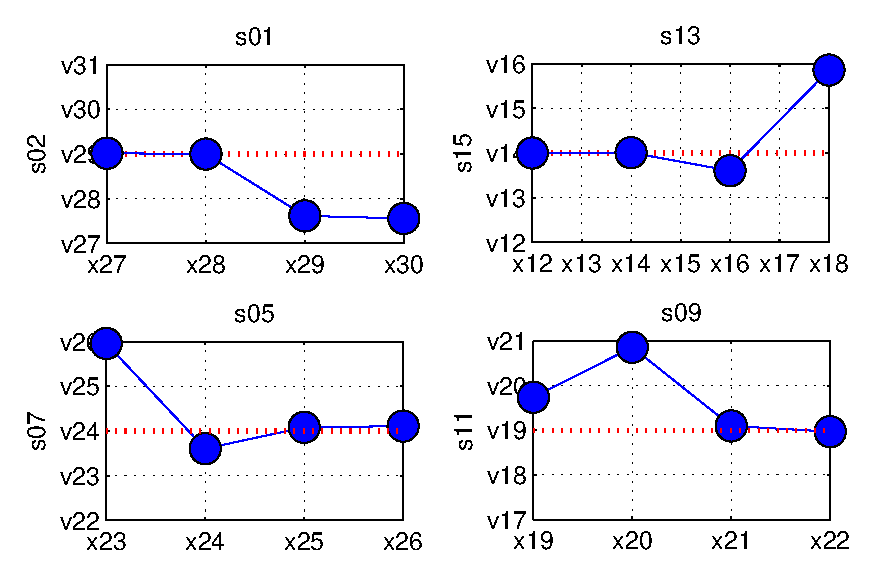
\includegraphics{./Figures/allmode.eps}}%
\end{psfrags}%
%
% End allmode.tex
\end{document}
% See http://www.mathworks.de/matlabcentral/fileexchange/loadFile.do?objectId=4638
% for recent versions of laprint.m.
%
% created by:           LaPrint version 3.16 (13.9.2004)
% created on:           05-Jan-2014 21:04:15
% eps bounding box:     15 cm x 8.8506 cm
% comment:              
%
\begin{psfrags}%
\psfragscanon%
%
% text strings:
\psfrag{s01}[b][b]{\color[rgb]{0,0,0}\setlength{\tabcolsep}{0pt}\begin{tabular}{c}mode 1\end{tabular}}%
\psfrag{s02}[b][b]{\color[rgb]{0,0,0}\setlength{\tabcolsep}{0pt}\begin{tabular}{c}relative displacement\end{tabular}}%
\psfrag{s05}[b][b]{\color[rgb]{0,0,0}\setlength{\tabcolsep}{0pt}\begin{tabular}{c}mode 3\end{tabular}}%
\psfrag{s07}[b][b]{\color[rgb]{0,0,0}\setlength{\tabcolsep}{0pt}\begin{tabular}{c}relative displacement\end{tabular}}%
\psfrag{s09}[b][b]{\color[rgb]{0,0,0}\setlength{\tabcolsep}{0pt}\begin{tabular}{c}mode 4\end{tabular}}%
\psfrag{s11}[b][b]{\color[rgb]{0,0,0}\setlength{\tabcolsep}{0pt}\begin{tabular}{c}relative displacement\end{tabular}}%
\psfrag{s13}[b][b]{\color[rgb]{0,0,0}\setlength{\tabcolsep}{0pt}\begin{tabular}{c}mode 2\end{tabular}}%
\psfrag{s15}[b][b]{\color[rgb]{0,0,0}\setlength{\tabcolsep}{0pt}\begin{tabular}{c}relative displacement\end{tabular}}%
%
% xticklabels:
\psfrag{x01}[t][t]{0}%
\psfrag{x02}[t][t]{0.1}%
\psfrag{x03}[t][t]{0.2}%
\psfrag{x04}[t][t]{0.3}%
\psfrag{x05}[t][t]{0.4}%
\psfrag{x06}[t][t]{0.5}%
\psfrag{x07}[t][t]{0.6}%
\psfrag{x08}[t][t]{0.7}%
\psfrag{x09}[t][t]{0.8}%
\psfrag{x10}[t][t]{0.9}%
\psfrag{x11}[t][t]{1}%
\psfrag{x12}[t][t]{1}%
\psfrag{x13}[t][t]{1.5}%
\psfrag{x14}[t][t]{2}%
\psfrag{x15}[t][t]{2.5}%
\psfrag{x16}[t][t]{3}%
\psfrag{x17}[t][t]{3.5}%
\psfrag{x18}[t][t]{4}%
\psfrag{x19}[t][t]{1}%
\psfrag{x20}[t][t]{2}%
\psfrag{x21}[t][t]{3}%
\psfrag{x22}[t][t]{4}%
\psfrag{x23}[t][t]{1}%
\psfrag{x24}[t][t]{2}%
\psfrag{x25}[t][t]{3}%
\psfrag{x26}[t][t]{4}%
\psfrag{x27}[t][t]{1}%
\psfrag{x28}[t][t]{2}%
\psfrag{x29}[t][t]{3}%
\psfrag{x30}[t][t]{4}%
%
% yticklabels:
\psfrag{v01}[r][r]{0}%
\psfrag{v02}[r][r]{0.1}%
\psfrag{v03}[r][r]{0.2}%
\psfrag{v04}[r][r]{0.3}%
\psfrag{v05}[r][r]{0.4}%
\psfrag{v06}[r][r]{0.5}%
\psfrag{v07}[r][r]{0.6}%
\psfrag{v08}[r][r]{0.7}%
\psfrag{v09}[r][r]{0.8}%
\psfrag{v10}[r][r]{0.9}%
\psfrag{v11}[r][r]{1}%
\psfrag{v12}[r][r]{-1}%
\psfrag{v13}[r][r]{-0.5}%
\psfrag{v14}[r][r]{0}%
\psfrag{v15}[r][r]{0.5}%
\psfrag{v16}[r][r]{1}%
\psfrag{v17}[r][r]{-1}%
\psfrag{v18}[r][r]{-0.5}%
\psfrag{v19}[r][r]{0}%
\psfrag{v20}[r][r]{0.5}%
\psfrag{v21}[r][r]{1}%
\psfrag{v22}[r][r]{-1}%
\psfrag{v23}[r][r]{-0.5}%
\psfrag{v24}[r][r]{0}%
\psfrag{v25}[r][r]{0.5}%
\psfrag{v26}[r][r]{1}%
\psfrag{v27}[r][r]{-1}%
\psfrag{v28}[r][r]{-0.5}%
\psfrag{v29}[r][r]{0}%
\psfrag{v30}[r][r]{0.5}%
\psfrag{v31}[r][r]{1}%
%
% Figure:
\resizebox{12cm}{!}{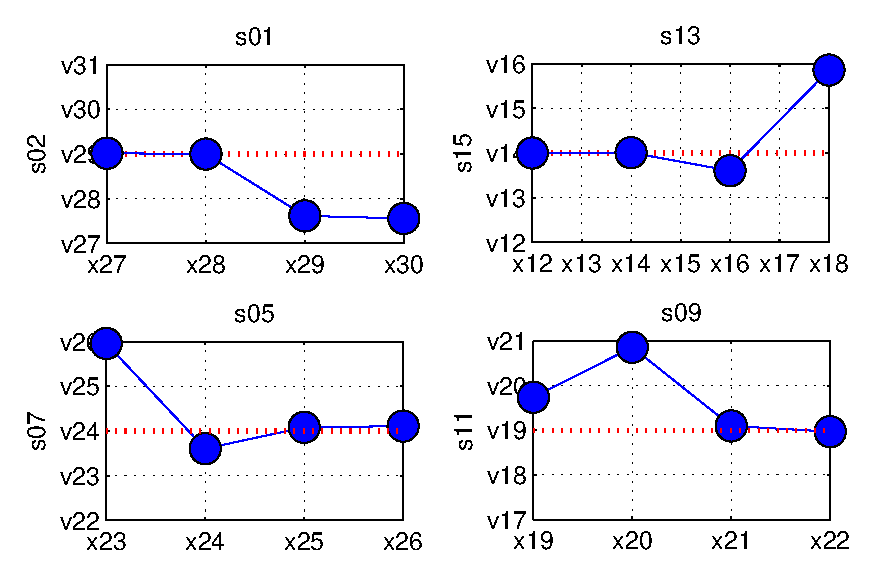
\includegraphics{./Figures/allmode.eps}}%
\end{psfrags}%
%
% End allmode.tex

\caption{Vibration modes}
\label{fig:allmodes}
\end{figure}
\newpage
~\\
\textbf{Compute modal mass and stiffness matrices.}
\\~\\
Modal mass and stiffness matrices are found from the relations
\begin{eqnarray*}
\mathbf{m}=\mathbf{\Phi}^T \mathbf{M} \mathbf{\Phi} \\
\mathbf{k}=\mathbf{\Phi}^T \mathbf{K} \mathbf{\Phi}
\end{eqnarray*}
where $\mathbf{\Phi}$ is the eigen modes matrix. If we calculate them it is found that
\begin{eqnarray*}
\mathbf{m}=\left(\begin{array}{cccc} 53.0 & 0 & 0 & 0\\ 0 & 53.0 & 0 & 0\\ 0 & 0 & 434.0 & 0\\ 0 & 0 & 0 & 764.0 \end{array}\right)
\end{eqnarray*}
and
\begin{eqnarray*}
\mathbf{k}=\left(\begin{array}{cccc} 2.1\cdot 10^5 & 0 & 0 & 0\\ 0 & 2.1\cdot 10^5 & 0 & 0\\ 0 & 0 & 1.98\cdot 10^4 & 0\\ 0 & 0 & 0 & 3.24\cdot 10^4 \end{array}\right)
\end{eqnarray*}
\newpage
~\\
\textbf{Show that vibration modes are orthogonal to each other with respect to mass and stiffness matrices.}
\\~\\
Zero bidiagonal elements in modal and stiffness matrices mean that the modes are orthogonal to each other with respect to mass and stiffness matrices. It is already showed that they are equal to zero in the previous answer.
\subsection*{Question 2}
\textbf{Suppose that while moving with a speed $\mathrm{V} = 60 km/h$ the right tire passes over a half sine wave-like bump on the road as shown below, where $\mathrm{a} = 30cm$ and $\mathrm{b} = 5cm$. Assuming zero initial conditions plot the 5 seconds responses of the coordinates $x_1$ and $x_2$.}
\begin{center}
\subsection*{Solution 2}
\end{center}
This problem can be solved numerically integrating the equations of motion. Before we do that, applied force on the second tire should be calculated. The force on the tire depends on the displacement of the road. Therefore, displacement profile with respect to time is
\begin{eqnarray*}
\mathrm{T}&= &0.072\frac{\mathrm{a}}{\mathrm{V}}\quad \mathrm{(seconds)}
\\
y_2&=&\{\begin{array}{clc}
\mathrm{b}\sin\left(\frac{2\pi}{\mathrm{T}}t\right) &,& 0\leq t \leq \frac{\mathrm{T}}{2} \\ 
0 &,& \frac{\mathrm{T}}{2}<t
\end{array}
\end{eqnarray*}
with the found displacement of the road, complete force vector of the model is found as
\begin{eqnarray*}
\mathrm{F}=\left[\begin{array}{ccc}
0\\
0\\
y_1 k_t\\
y_2 k_t
\end{array}\right]
\end{eqnarray*}
With this calculated road input force, a numerical solution to the equations of motion of the car is done by a matlab function. This function is given in~\cref{lst:odefunc} and it calculates required derivatives of the system by using order reducing method. The derivatives can be integrated by a numerical method, for example Runge-Kutta. For the integration of derivatives \mcode{Ode45} function of matlab is used in which integration is done with Runge-Kutta45 method. Integration is completed with the command in \cref{lst:command}.
\lstset{frame=single,numbers=left}
\begin{lstlisting}[label=lst:command,caption=integration commands]
options = odeset('MaxStep',1e-3)
[t y]=ode45(@odefunc,[0 5],[0 0 0 0 0 0 0 0],options);
\end{lstlisting}
%\begin{eqnarray*}
%{{\mathbf M}}\mathbf{\ddot {\mathbf x}}+{{\mathbf C}}\mathbf{\dot {\mathbf x}}+{{\mathbf K}}\mathbf{ {\mathbf x}}={{\mathbf F}}
%\end{eqnarray*}
\newpage
\lstset{frame=single,numbers=left}
\lstinputlisting[label=lst:odefunc,caption={{odefunc.m}}]{Matlab/odefunc.m}
Using \cref{lst:command} with \cref{lst:odefunc} the resulting time dependent behaviors of the displacements of the right and the left tires are given in \cref{fig:timedependenttires}.
\begin{figure}[ht!]
\centering
% This file is generated by the MATLAB m-file laprint.m. It can be included
% into LaTeX documents using the packages graphicx, color and psfrag.
% It is accompanied by a postscript file. A sample LaTeX file is:
%    \documentclass{article}\usepackage{graphicx,color,psfrag}
%    \begin{document}% This file is generated by the MATLAB m-file laprint.m. It can be included
% into LaTeX documents using the packages graphicx, color and psfrag.
% It is accompanied by a postscript file. A sample LaTeX file is:
%    \documentclass{article}\usepackage{graphicx,color,psfrag}
%    \begin{document}% This file is generated by the MATLAB m-file laprint.m. It can be included
% into LaTeX documents using the packages graphicx, color and psfrag.
% It is accompanied by a postscript file. A sample LaTeX file is:
%    \documentclass{article}\usepackage{graphicx,color,psfrag}
%    \begin{document}\input{timedependent}\end{document}
% See http://www.mathworks.de/matlabcentral/fileexchange/loadFile.do?objectId=4638
% for recent versions of laprint.m.
%
% created by:           LaPrint version 3.16 (13.9.2004)
% created on:           07-Jan-2014 16:25:10
% eps bounding box:     15 cm x 9.1251 cm
% comment:              
%
\begin{psfrags}%
\psfragscanon%
%
% text strings:
\psfrag{s01}[t][t]{\color[rgb]{0,0,0}\setlength{\tabcolsep}{0pt}\begin{tabular}{c}time [seconds]\end{tabular}}%
\psfrag{s02}[b][b]{\color[rgb]{0,0,0}\setlength{\tabcolsep}{0pt}\begin{tabular}{c}displacement [cm]\end{tabular}}%
\psfrag{s04}[b][b]{\color[rgb]{0,0,0}\setlength{\tabcolsep}{0pt}\begin{tabular}{c}right tire\end{tabular}}%
\psfrag{s05}[b][b]{\color[rgb]{0,0,0}\setlength{\tabcolsep}{0pt}\begin{tabular}{c}left tire\end{tabular}}%
\psfrag{s06}[t][t]{\color[rgb]{0,0,0}\setlength{\tabcolsep}{0pt}\begin{tabular}{c}time [seconds]\end{tabular}}%
\psfrag{s07}[b][b]{\color[rgb]{0,0,0}\setlength{\tabcolsep}{0pt}\begin{tabular}{c}displacement [cm]\end{tabular}}%
%
% xticklabels:
\psfrag{x01}[t][t]{0}%
\psfrag{x02}[t][t]{0.1}%
\psfrag{x03}[t][t]{0.2}%
\psfrag{x04}[t][t]{0.3}%
\psfrag{x05}[t][t]{0.4}%
\psfrag{x06}[t][t]{0.5}%
\psfrag{x07}[t][t]{0.6}%
\psfrag{x08}[t][t]{0.7}%
\psfrag{x09}[t][t]{0.8}%
\psfrag{x10}[t][t]{0.9}%
\psfrag{x11}[t][t]{1}%
\psfrag{x12}[t][t]{0}%
\psfrag{x13}[t][t]{0.5}%
\psfrag{x14}[t][t]{1}%
\psfrag{x15}[t][t]{1.5}%
\psfrag{x16}[t][t]{2}%
\psfrag{x17}[t][t]{2.5}%
\psfrag{x18}[t][t]{3}%
\psfrag{x19}[t][t]{3.5}%
\psfrag{x20}[t][t]{4}%
\psfrag{x21}[t][t]{4.5}%
\psfrag{x22}[t][t]{5}%
\psfrag{x23}[t][t]{0}%
\psfrag{x24}[t][t]{0.5}%
\psfrag{x25}[t][t]{1}%
\psfrag{x26}[t][t]{1.5}%
\psfrag{x27}[t][t]{2}%
\psfrag{x28}[t][t]{2.5}%
\psfrag{x29}[t][t]{3}%
\psfrag{x30}[t][t]{3.5}%
\psfrag{x31}[t][t]{4}%
\psfrag{x32}[t][t]{4.5}%
\psfrag{x33}[t][t]{5}%
%
% yticklabels:
\psfrag{v01}[r][r]{0}%
\psfrag{v02}[r][r]{0.1}%
\psfrag{v03}[r][r]{0.2}%
\psfrag{v04}[r][r]{0.3}%
\psfrag{v05}[r][r]{0.4}%
\psfrag{v06}[r][r]{0.5}%
\psfrag{v07}[r][r]{0.6}%
\psfrag{v08}[r][r]{0.7}%
\psfrag{v09}[r][r]{0.8}%
\psfrag{v10}[r][r]{0.9}%
\psfrag{v11}[r][r]{1}%
\psfrag{v12}[r][r]{    -0.02}%
\psfrag{v13}[r][r]{   -0.015}%
\psfrag{v14}[r][r]{    -0.01}%
\psfrag{v15}[r][r]{-0.005}%
\psfrag{v16}[r][r]{0}%
\psfrag{v17}[r][r]{0.005}%
\psfrag{v18}[r][r]{     0.01}%
\psfrag{v19}[r][r]{    0.015}%
\psfrag{v20}[r][r]{-3}%
\psfrag{v21}[r][r]{-2}%
\psfrag{v22}[r][r]{-1}%
\psfrag{v23}[r][r]{0}%
\psfrag{v24}[r][r]{1}%
\psfrag{v25}[r][r]{2}%
\psfrag{v26}[r][r]{3}%
\psfrag{v27}[r][r]{4}%
%
% Figure:
\resizebox{12cm}{!}{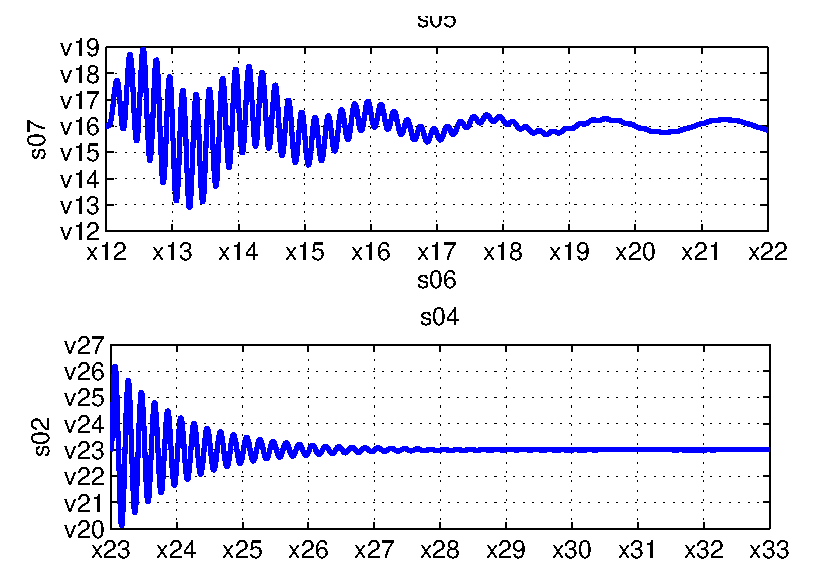
\includegraphics{./Figures/timedependent.eps}}%
\end{psfrags}%
%
% End timedependent.tex
\end{document}
% See http://www.mathworks.de/matlabcentral/fileexchange/loadFile.do?objectId=4638
% for recent versions of laprint.m.
%
% created by:           LaPrint version 3.16 (13.9.2004)
% created on:           07-Jan-2014 16:25:10
% eps bounding box:     15 cm x 9.1251 cm
% comment:              
%
\begin{psfrags}%
\psfragscanon%
%
% text strings:
\psfrag{s01}[t][t]{\color[rgb]{0,0,0}\setlength{\tabcolsep}{0pt}\begin{tabular}{c}time [seconds]\end{tabular}}%
\psfrag{s02}[b][b]{\color[rgb]{0,0,0}\setlength{\tabcolsep}{0pt}\begin{tabular}{c}displacement [cm]\end{tabular}}%
\psfrag{s04}[b][b]{\color[rgb]{0,0,0}\setlength{\tabcolsep}{0pt}\begin{tabular}{c}right tire\end{tabular}}%
\psfrag{s05}[b][b]{\color[rgb]{0,0,0}\setlength{\tabcolsep}{0pt}\begin{tabular}{c}left tire\end{tabular}}%
\psfrag{s06}[t][t]{\color[rgb]{0,0,0}\setlength{\tabcolsep}{0pt}\begin{tabular}{c}time [seconds]\end{tabular}}%
\psfrag{s07}[b][b]{\color[rgb]{0,0,0}\setlength{\tabcolsep}{0pt}\begin{tabular}{c}displacement [cm]\end{tabular}}%
%
% xticklabels:
\psfrag{x01}[t][t]{0}%
\psfrag{x02}[t][t]{0.1}%
\psfrag{x03}[t][t]{0.2}%
\psfrag{x04}[t][t]{0.3}%
\psfrag{x05}[t][t]{0.4}%
\psfrag{x06}[t][t]{0.5}%
\psfrag{x07}[t][t]{0.6}%
\psfrag{x08}[t][t]{0.7}%
\psfrag{x09}[t][t]{0.8}%
\psfrag{x10}[t][t]{0.9}%
\psfrag{x11}[t][t]{1}%
\psfrag{x12}[t][t]{0}%
\psfrag{x13}[t][t]{0.5}%
\psfrag{x14}[t][t]{1}%
\psfrag{x15}[t][t]{1.5}%
\psfrag{x16}[t][t]{2}%
\psfrag{x17}[t][t]{2.5}%
\psfrag{x18}[t][t]{3}%
\psfrag{x19}[t][t]{3.5}%
\psfrag{x20}[t][t]{4}%
\psfrag{x21}[t][t]{4.5}%
\psfrag{x22}[t][t]{5}%
\psfrag{x23}[t][t]{0}%
\psfrag{x24}[t][t]{0.5}%
\psfrag{x25}[t][t]{1}%
\psfrag{x26}[t][t]{1.5}%
\psfrag{x27}[t][t]{2}%
\psfrag{x28}[t][t]{2.5}%
\psfrag{x29}[t][t]{3}%
\psfrag{x30}[t][t]{3.5}%
\psfrag{x31}[t][t]{4}%
\psfrag{x32}[t][t]{4.5}%
\psfrag{x33}[t][t]{5}%
%
% yticklabels:
\psfrag{v01}[r][r]{0}%
\psfrag{v02}[r][r]{0.1}%
\psfrag{v03}[r][r]{0.2}%
\psfrag{v04}[r][r]{0.3}%
\psfrag{v05}[r][r]{0.4}%
\psfrag{v06}[r][r]{0.5}%
\psfrag{v07}[r][r]{0.6}%
\psfrag{v08}[r][r]{0.7}%
\psfrag{v09}[r][r]{0.8}%
\psfrag{v10}[r][r]{0.9}%
\psfrag{v11}[r][r]{1}%
\psfrag{v12}[r][r]{    -0.02}%
\psfrag{v13}[r][r]{   -0.015}%
\psfrag{v14}[r][r]{    -0.01}%
\psfrag{v15}[r][r]{-0.005}%
\psfrag{v16}[r][r]{0}%
\psfrag{v17}[r][r]{0.005}%
\psfrag{v18}[r][r]{     0.01}%
\psfrag{v19}[r][r]{    0.015}%
\psfrag{v20}[r][r]{-3}%
\psfrag{v21}[r][r]{-2}%
\psfrag{v22}[r][r]{-1}%
\psfrag{v23}[r][r]{0}%
\psfrag{v24}[r][r]{1}%
\psfrag{v25}[r][r]{2}%
\psfrag{v26}[r][r]{3}%
\psfrag{v27}[r][r]{4}%
%
% Figure:
\resizebox{12cm}{!}{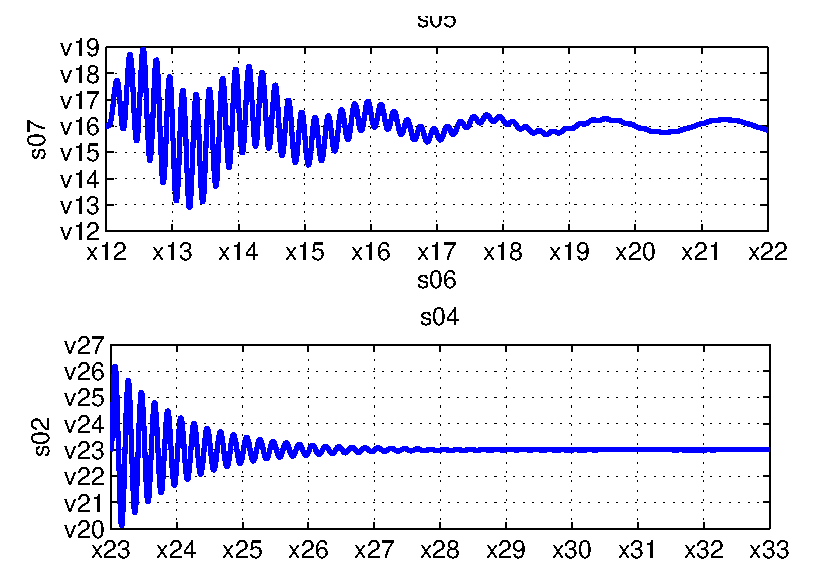
\includegraphics{./Figures/timedependent.eps}}%
\end{psfrags}%
%
% End timedependent.tex
\end{document}
% See http://www.mathworks.de/matlabcentral/fileexchange/loadFile.do?objectId=4638
% for recent versions of laprint.m.
%
% created by:           LaPrint version 3.16 (13.9.2004)
% created on:           07-Jan-2014 16:25:10
% eps bounding box:     15 cm x 9.1251 cm
% comment:              
%
\begin{psfrags}%
\psfragscanon%
%
% text strings:
\psfrag{s01}[t][t]{\color[rgb]{0,0,0}\setlength{\tabcolsep}{0pt}\begin{tabular}{c}time [seconds]\end{tabular}}%
\psfrag{s02}[b][b]{\color[rgb]{0,0,0}\setlength{\tabcolsep}{0pt}\begin{tabular}{c}displacement [cm]\end{tabular}}%
\psfrag{s04}[b][b]{\color[rgb]{0,0,0}\setlength{\tabcolsep}{0pt}\begin{tabular}{c}right tire\end{tabular}}%
\psfrag{s05}[b][b]{\color[rgb]{0,0,0}\setlength{\tabcolsep}{0pt}\begin{tabular}{c}left tire\end{tabular}}%
\psfrag{s06}[t][t]{\color[rgb]{0,0,0}\setlength{\tabcolsep}{0pt}\begin{tabular}{c}time [seconds]\end{tabular}}%
\psfrag{s07}[b][b]{\color[rgb]{0,0,0}\setlength{\tabcolsep}{0pt}\begin{tabular}{c}displacement [cm]\end{tabular}}%
%
% xticklabels:
\psfrag{x01}[t][t]{0}%
\psfrag{x02}[t][t]{0.1}%
\psfrag{x03}[t][t]{0.2}%
\psfrag{x04}[t][t]{0.3}%
\psfrag{x05}[t][t]{0.4}%
\psfrag{x06}[t][t]{0.5}%
\psfrag{x07}[t][t]{0.6}%
\psfrag{x08}[t][t]{0.7}%
\psfrag{x09}[t][t]{0.8}%
\psfrag{x10}[t][t]{0.9}%
\psfrag{x11}[t][t]{1}%
\psfrag{x12}[t][t]{0}%
\psfrag{x13}[t][t]{0.5}%
\psfrag{x14}[t][t]{1}%
\psfrag{x15}[t][t]{1.5}%
\psfrag{x16}[t][t]{2}%
\psfrag{x17}[t][t]{2.5}%
\psfrag{x18}[t][t]{3}%
\psfrag{x19}[t][t]{3.5}%
\psfrag{x20}[t][t]{4}%
\psfrag{x21}[t][t]{4.5}%
\psfrag{x22}[t][t]{5}%
\psfrag{x23}[t][t]{0}%
\psfrag{x24}[t][t]{0.5}%
\psfrag{x25}[t][t]{1}%
\psfrag{x26}[t][t]{1.5}%
\psfrag{x27}[t][t]{2}%
\psfrag{x28}[t][t]{2.5}%
\psfrag{x29}[t][t]{3}%
\psfrag{x30}[t][t]{3.5}%
\psfrag{x31}[t][t]{4}%
\psfrag{x32}[t][t]{4.5}%
\psfrag{x33}[t][t]{5}%
%
% yticklabels:
\psfrag{v01}[r][r]{0}%
\psfrag{v02}[r][r]{0.1}%
\psfrag{v03}[r][r]{0.2}%
\psfrag{v04}[r][r]{0.3}%
\psfrag{v05}[r][r]{0.4}%
\psfrag{v06}[r][r]{0.5}%
\psfrag{v07}[r][r]{0.6}%
\psfrag{v08}[r][r]{0.7}%
\psfrag{v09}[r][r]{0.8}%
\psfrag{v10}[r][r]{0.9}%
\psfrag{v11}[r][r]{1}%
\psfrag{v12}[r][r]{    -0.02}%
\psfrag{v13}[r][r]{   -0.015}%
\psfrag{v14}[r][r]{    -0.01}%
\psfrag{v15}[r][r]{-0.005}%
\psfrag{v16}[r][r]{0}%
\psfrag{v17}[r][r]{0.005}%
\psfrag{v18}[r][r]{     0.01}%
\psfrag{v19}[r][r]{    0.015}%
\psfrag{v20}[r][r]{-3}%
\psfrag{v21}[r][r]{-2}%
\psfrag{v22}[r][r]{-1}%
\psfrag{v23}[r][r]{0}%
\psfrag{v24}[r][r]{1}%
\psfrag{v25}[r][r]{2}%
\psfrag{v26}[r][r]{3}%
\psfrag{v27}[r][r]{4}%
%
% Figure:
\resizebox{12cm}{!}{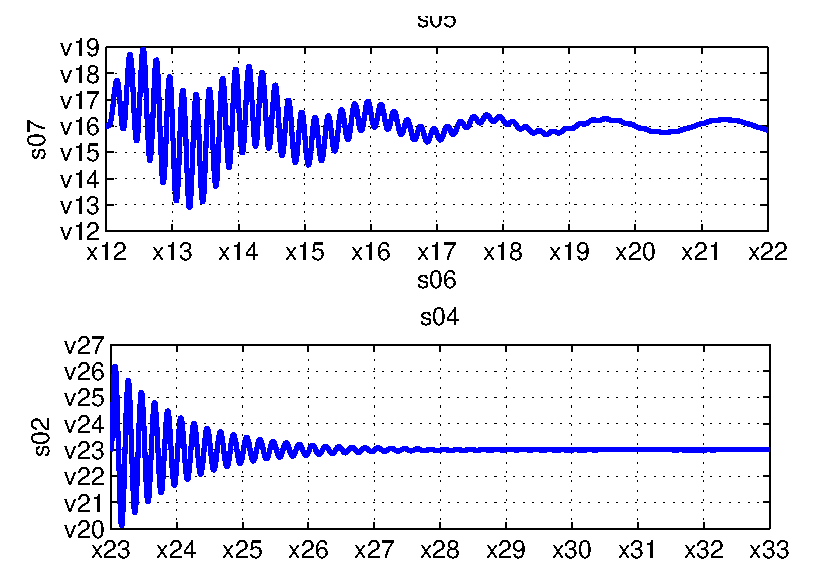
\includegraphics{./Figures/timedependent.eps}}%
\end{psfrags}%
%
% End timedependent.tex

\caption{Time dependent motion of the tires of the car.}
\label{fig:timedependenttires}
\end{figure}

\section*{Problem 2}
In \cref{fig:problem2}, a beam  with fixed one end, carrying  a rigid tip mass M , and exhibits transverse vibrations is given. Physical properties are as follows:  $L =1m$, $E=210GPa$, $\rho=7800kgm^{-3}$, sizes of the rectangular cross section $a=2cm$ $b=1cm$, $M$ is twice of the beam mass.
\begin{figure}[ht!]
\centering
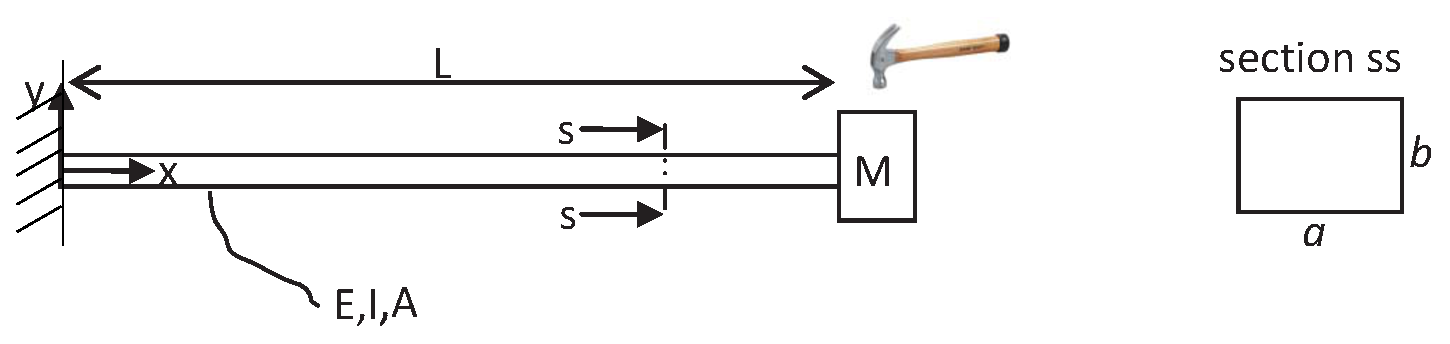
\includegraphics[width=\textwidth]{./Figures/2st_Assignment_2}
\caption{Problem 2}
\label{fig:problem2}
\end{figure}
\subsection*{Question 1}
\textbf{Derive the equations of motion with suitable boundary conditions.}
\begin{center}
\subsection*{Solution 1}
\end{center}
The transverse equation of motion for the beam is given by
\begin{eqnarray*}
 EI~\cfrac{\partial^4 w}{\partial x^4} + \rho A~\cfrac{\partial^2 w}{\partial t^2} = 0
\end{eqnarray*}
The boundary conditions for the problem are as follows:\\
\begin{enumerate}
\item {zero displacement at $x=0$ :\\ \begin{eqnarray*}
w\left(0,t\right)=0
\end{eqnarray*} }
\item {zero slope of displacement at $x=0$ :\\ \begin{eqnarray*}
\cfrac{\partial w\left(0,t\right)}{\partial x}=0
\end{eqnarray*} }
\item {shear force acceleration of lumped mass equilibrium at $x=L$ :\\ \begin{eqnarray*}
 EI~\cfrac{\partial w^3\left(L,t\right)}{\partial x^3}=M\cfrac{\partial w^2\left(L,t\right)}{\partial t^2}
\end{eqnarray*} }
\item {zero moment at $x=L$ :\\ \begin{eqnarray*}
 EI~\cfrac{\partial w^2\left(L,t\right)}{\partial x^2}=0
\end{eqnarray*} }
\end{enumerate}
\subsection*{Question 2}
\textbf{Find the first five natural frequencies (Hz) and vibration modes of the system. Plot the vibration modes in the same figure.}
\begin{center}
\subsection*{Solution 2}
\end{center}
Using seperation of variables method, the displacements of the beam can be written as
\begin{eqnarray*}
u\left(x,t\right)=U\left(x\right)T\left(t\right)
\end{eqnarray*}
using this assumption with the equations of motion we have
\begin{eqnarray*}
U^{IV} +\lambda^4U&=&0\\
\ddot{T} +\omega^2 T&=&0
\end{eqnarray*}
Using these differential equations , the space dependent part of the solution of transverse vibration of beam is found as
\begin{eqnarray*}
X(x)=A\cosh\left(\cfrac{\lambda x}{L}\right)+B\sinh\left(\cfrac{\lambda x}{L}\right)+C\cos\left(\cfrac{\lambda x}{L}\right)+D\sin\left(\cfrac{\lambda x}{L}\right)
\end{eqnarray*}
and time dependent part as
\begin{eqnarray*}
X(x)=\bar{A}\cos\left({\omega t}\right)+\bar{B}\sin\left({\omega t}\right)
\end{eqnarray*}
where $\omega^2=\lambda^4 \cfrac{EI}{mL^4}$. In these equations have 4 variables to determine in the space dependent part. Using boundary conditions, these variables can be determined. Using first two boundary conditions
\begin{eqnarray*}
U\left(0,t\right)= 0 &;&  A+C=0 \quad \Longrightarrow \quad A=-C\\
U'\left(0,t\right)= 0&;& B+D=0 \quad \Longrightarrow \quad B=-D
\end{eqnarray*}
Using other boundary conditions
\begin{eqnarray*}
EIU''\left(L,t\right)= 0&;& A\biggl[\cosh\left(\lambda \right)+\cos\left(\lambda \right)\biggl]+
B\biggl[\sinh\left(\lambda \right)+\sin\left(\lambda \right)\biggr]=0\\
EIU'''\left(L,t\right)-M\omega^2U\left(L,t\right)= 0&;& A\underbrace{\biggl[EI\left(\cfrac{\lambda}{L}\right)^3\left(\sinh\left(\lambda \right)-\sin\left(\lambda \right)\right)+ \quad M\omega^2\left(\cosh\left(\lambda \right)-\cos\left(\lambda \right)\right)\biggr]}_{\xi_A}+\\
&&
\underbrace{\biggl[EI\left(\cfrac{\lambda}{L}\right)^3\left(\cosh\left(\lambda \right)+\cos\left(\lambda \right)\right) \quad M\omega^2\left(\sinh\left(\lambda \right)-\sin\left(\lambda \right)\right)\biggr]}_{\xi_B}=0
\end{eqnarray*}
These two equations with two unknowns can be written as
\begin{eqnarray*}
\left[\begin{array}{cc}
\cosh\left(\lambda \right)+\cos\left(\lambda \right)&\sinh\left(\lambda \right)+\sin\left(\lambda \right) \\
\xi_A & \xi_B\end{array}\right]=\left[\begin{array}{c}
A\\B
\end{array}\right]=\mathbf{0}
\end{eqnarray*}
where determinant of the coefficient matrix must be zero for a meaningful solution of the variables. This results the equation
\begin{eqnarray*}
\left(E\, I\, {\lambda}^3\, \left(\cos\!\left(\lambda\right) + \cosh\!\left(\lambda\right)\right) - \frac{E\, I\, M\, {\lambda}^4\, \sinh\!\left(\sin\!\left(\lambda\right) - \lambda\right)}{L^4\, m}\right)\, \left(\cos\!\left(\lambda\right) + \cosh\!\left(\lambda\right)\right) - \left(E\, I\, {\lambda}^3\, \left(\sin\!\left(\lambda\right) + \sinh\!\left(\lambda\right)\right) + \frac{E\, I\, M\, {\lambda}^4\, \cosh\!\left(\cos\!\left(\lambda\right) - \lambda\right)}{L^4\, m}\right)\, \left(\sin\!\left(\lambda\right) + \sinh\!\left(\lambda\right)\right)
\end{eqnarray*}


\bibliographystyle{plain}
\bibliography{biblio}

\end{document}          


